\documentclass{article}

% Language setting
% Replace `english' with e.g. `spanish' to change the document language
\usepackage[english]{babel}

% Set page size and margins
% Replace `letterpaper' with `a4paper' for UK/EU standard size
\usepackage[a4paper,top=2cm,bottom=2cm,left=3cm,right=3cm,marginparwidth=1.75cm]{geometry}

% Useful packages
\usepackage{amsmath}
\usepackage{graphicx}
\usepackage[colorlinks=true, allcolors=blue]{hyperref}
\usepackage{xcolor}
\usepackage{listings}

\colorlet{mygray}{black!30}
\colorlet{mygreen}{green!60!blue}
\colorlet{mymauve}{red!60!blue}

\lstset{
  backgroundcolor=\color{gray!10},  
  basicstyle=\ttfamily,
  columns=fullflexible,
  breakatwhitespace=false,      
  breaklines=true,                
  captionpos=b,                    
  commentstyle=\color{mygreen}, 
  extendedchars=true,              
  frame=single,                   
  keepspaces=true,             
  keywordstyle=\color{blue},      
  language=c++,                 
  numbers=none,                
  numbersep=5pt,                   
  numberstyle=\tiny\color{blue}, 
  rulecolor=\color{mygray},        
  showspaces=false,
  showstringspaces=false,
  showtabs=false,                 
  stepnumber=5,                  
  stringstyle=\color{mymauve},    
  tabsize=3,                                     
  title=\lstname 
}


\lstnewenvironment{code}[2][]{%
  \lstset{%
    numbers = left,
    title   = #2,
    #1,
  }%
}{}

\title{Homework 4}
\author{Steinarr Hrafn Höskuldsson}

\newcommand{\mycomment}[1]{}
\usepackage{fancyhdr}
\fancypagestyle{firststyle}
{
   \fancyhf{}
   \fancyhead[L]{Mechatronics 2}
   
   \renewcommand{\headrulewidth}{0pt} % removes horizontal header line
}
\begin{document}

\mycomment{

\begin{figure}[h]
    \centering
    \includegraphics[width=0.75\textwidth]{LAB3/Basic1.png}
    \caption{"Switch test" Breadboard set up}
    \label{fig:Switch_test}
\end{figure}

\lstinputlisting[caption=Defining 'ColorMatch' state, label={lst:colormatch}, language=Python, firstline=44, lastline=52]{LAB3/Basic.py}

} % end of comment

\pagestyle{firststyle}
{\let\newpage\relax\maketitle}

\section{Homemade Delay Library}
Source and header files were created for the library which is designed for code compiled with Heavy Optimization. 

To delay 1 microsecond, 16 clock cycles must be burned off. It is rather convenient that the \verb"call" instruction and \verb"ret" instruction both take 4 clock cycles to execute so a function that takes no parameters and returns immediately takes 8 clock cycles to run, exactly half a microsecond.

So a half microsecond delay could be implemented as
\begin{lstlisting}
void delay_half_us()
{
	// nothing
}   
\end{lstlisting}
To test if this actually burns half a microsecond a test was devised writing a simple main program:

\begin{lstlisting}
int main()
{
	DDRB |= 0x20;
	while (1)
	{
		delay_half_us(); 	// 8 cycles
		PORTB = 0x20;		// 1 cycle
		delay_half_us();	// 8 cycles
		PORTB = 0;			// 1 cycle
	}				// loop -> 2 cycles
}					// 		== 20 cycles
\end{lstlisting}

Which, as the comments suggest should result in a square wave on pin D13 with period $20/16MHz = 1.25 \mu s$

And this was confirmed by oscilloscope as can be seen on Figure \ref{hw4:fig:scope1}

\begin{figure}
    \centering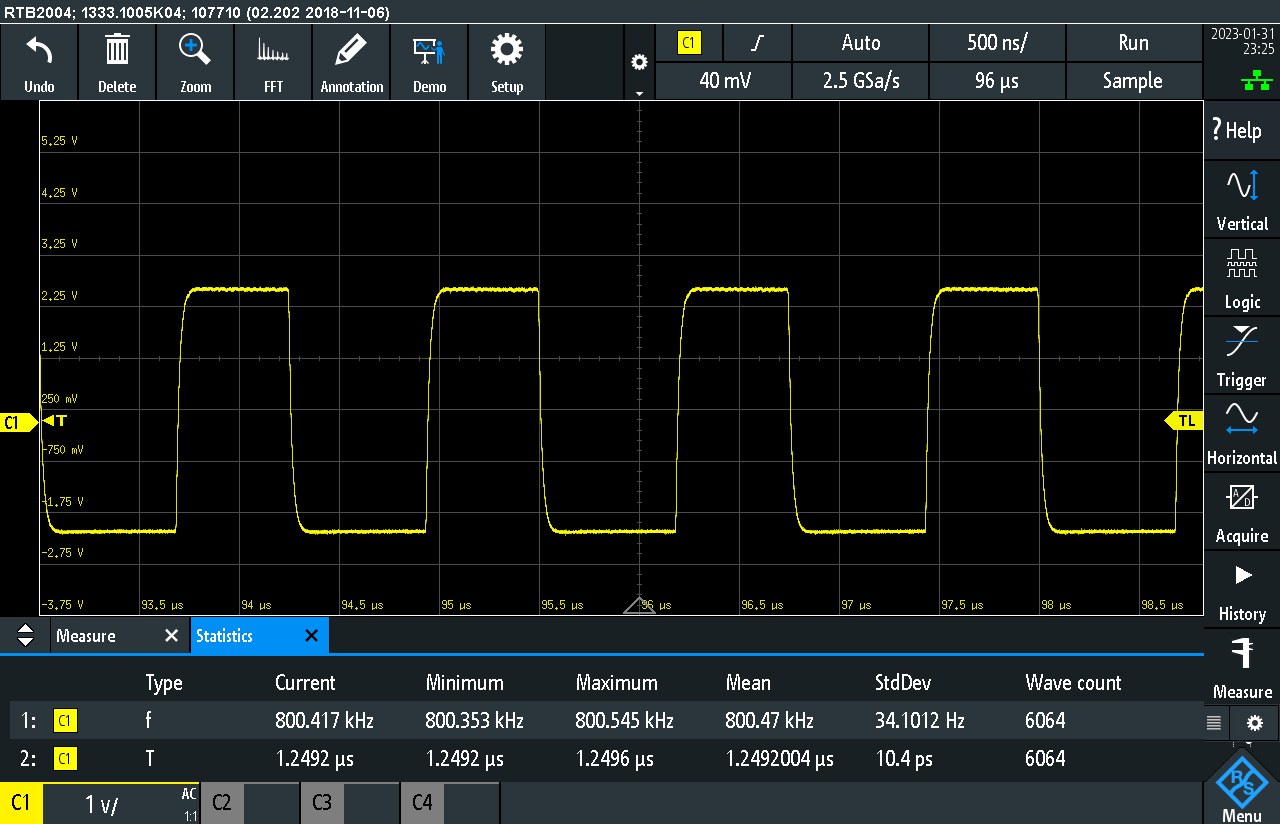
\includegraphics[width=\textwidth]{HW4/HW4Scope.png}
    \caption{Caption}
    \label{hw4:fig:scope1}
\end{figure}

Now let's look at creating a variable microsecond delay.
Some research yields that clock cycles can be burned off by using \verb!asm volatile("nop\n\t"::);!
and the volatile flag keeps the compiler from optimizing it out.

A function was devised with the overall structure of a loop counting down the \verb"us" variable where each loop takes exactly 16 cycles. The function would of course also have to deal with the cycles lost in the overhead of being called.

Such a function was written, the resulting assembly instructions were then analysed and the function edited until the overhead was accounted for and the loop took exactly 16 cycles. Here is the function, the comments speak for themselves.
\newpage
\begin{lstlisting}[caption={A function that burns exactly 'us' microseconds when called}]

void delay_us(unsigned int us)
{
	// overhead from calling function,
	// (2*ldi + call) costs 6 cycles

	// special case for us=1, (covers us=0 as well)
	// comparison costs 2 cycles (cpc and cpi)
	if (us < 2) // branches with brcs
	{
		// branch: 2 cycles to go here

		// at this point we are aiming for 1 microseconds
		// that is 16 cycles. We spent 6 on (2*ldi+call),
		// 2 on comparison, 2 on the branching and 4 for the return
		// leaving 16-6-4-2-2 = 2 cycles left to spend
		asm volatile("nop\n\t"
					 "nop\n\t"::);
		return; // 4 cycles for ret
	}
	// branch: one cycle to go here

	// burn 2 cycles to make the overhead from
	// calling to be exactly 1 microsecond
	// see calculation for why 2 cycles at the bottom
	// of the function
	asm volatile("nop\n\t"
                "nop\n\t"::);
	// subtract the one microseconds that burns up
	// in the overhead
	us--; // takes 2 cycles (sbwi)

	// each loop should then be exactly 1 microsecond
	while(1)
	{
		// this loop should take 16 cycles,
		// so here we burn 16 -2 -2 = 12 cycles
		asm volatile("nop\n\t"
				 	 "nop\n\t"
					 "nop\n\t"
					 "nop\n\t"
					 "nop\n\t"
					 "nop\n\t"
					 "nop\n\t"
					 "nop\n\t"
					 "nop\n\t"
					 "nop\n\t"
					 "nop\n\t"
					 "nop\n\t"::);
		us--; // sbwi: 2 cycles, saves overflow to Zero Flag
		if (!us) // branches with brne
		{
			// 1 cycle to go here
			return; // 4 cycles
		}
		// 2 cycles to go here (aka to loop)
	}
	// Why 2 cycles:
	// Overhead from calling is:
	// 2*ldi+call	6 cycles
	// cpi + cpc	2 cycles
	// if (brcs)	1 cycle (didn't branch)
	// sbwi			2 cycles
	// return		4
	// and finally the last loop will take be one cycle
	// short of 1 microsecond because the brne instruction
	// takes 2 cycles if it branches as expected in the loop
	// but the last loop doesn't branch so brne only takes 1 cycle
	// leaving the last loop as only 15 cycles.

	// so the overhead should aim for 17 cycles to make
	// up that one cycle that gets forgotten in the last loop

	// so we have  17 = 6 + 4 + 2 + 2 + 1 + X
	// 			==> X = 2
}
\end{lstlisting}\label{hw4:code:delayus}

The variable microsecond delay was tested with the same method as before using oscilloscope for different values of \textbf{us} confirming that it works as designed.

The microsecond delay function was used as a template to write a millisecond delay function

However when trying to use the microsecond delay function inside the millisecond delay function it became clear that the compiler didn't use the call instruction as expected. Instead it added instructions that logically behaved the same but used other registers, and in turn other instructions that took a different amount of cycles. The compiler even optimized out the less than 2 check since it new it was irrelevant but in doing so messed up the cycle accounting.

At this stage it became clear that it would not be accurate to rely on the compiler and its enigmatic optimization priorities.

Therefore after many hours of testing out different methods and reading about asm and macros syntax, a new strategy was devised.

Two macros were written, \verb"DELAY_9P4(i)" which delays for $9 + 4*i$ cycles and \verb"DELAY_9P262153(i)" which delays for $9+262,153*i$ cycles.

Since they are macros they will just insert the assembly code into the function at the specified location, thus giving complete predictability of the behaviour.

The macros use registers 24 and 25 to count the loops and thus start by pushing them to the stack before looping and finally pop them back from the stack after the looping. The macros do affect the status registers, but that was found to be acceptable.

\begin{lstlisting}
    
// Macro that delays for 9+4*us cycles
// push+push+ldi+ldi+pop+pop = 2+2+1+1+2+2 = 10 cycles
// loop is sbiw+brne = 2+2 = 4 cycles except the last one
// which is only 3, bringing the total to 9+4*us
#define DELAY_9P4(i) \
do { \
	asm volatile ("push r24"::);\
	asm volatile ("push r25"::);\
	asm volatile("ldi r25, %0"::"M"(i>>8));\
	asm volatile("ldi r24, %0"::"M"(i&0xff));\
	asm volatile("sbiw r24, 0x01");\
	asm volatile("brne .-4");\
	asm volatile ("pop r25"::);\
	asm volatile ("pop r24"::);\
} while (0)

//
// push+push+ldi+ldi+pop+pop = 2+2+1+1+2+2 = 10 cycles
// loop is sbiw+brne+(9+0xffff*4) = 2+2+9+4*65535 = 262.153 cycles
// except the last one which is one shorter,
// bringing the total to 9+262.153*us
#define DELAY_9P262153(i) \
do { \
	asm volatile ("push r24"::);\
	asm volatile ("push r25"::);\
	asm volatile("ldi r25, %0"::"M"(i>>8));\
	asm volatile("ldi r24, %0"::"M"(i&0xff));\
	DELAY_9P4(0xffff);\
	asm volatile("sbiw r24, 0x01");\
	asm volatile("brne .-20");\
	asm volatile ("pop r25"::);\
	asm volatile ("pop r24"::);\
} while (0)
\end{lstlisting}

Now a millisecond delay function and a second delay function could be written with the same structure as the microsecond delay function.

\begin{lstlisting}
    
void delay_ms(unsigned int ms)
{   // 6 cycles for call overhead

	// accounting for overhead:
	// goal here is total of 16.000 cycles or exactly 1 ms
	// so far we spent 6, comparison(<2) will take 2 cycles
	// the single nop will take 1 and jump to return will take 2
	// or the skip will take 1 and the decrement will take 2
	// the return will cost 4
	// for a total of 6 + 2 + 2 + 4 = 15
	// so now we should spend 16.000 - 15 = 15.985

	DELAY_9P4(3994); // takes 4*3.994 + 9 = 15.985

	// 2 cycles for comparison
	if (ms < 2)
	{// 2 cycles to get here

		// one nop here to equal the overhead branches
		asm volatile("nop\n\t");
		return;
	}
	// 1 cycle to get here
	ms--; // 2 cycles (sbiw)

	// this loop shall take 1 ms (16.000 cycles) per loop
	while(1)
	{
		// accounting for this loop
		// sbiw and brne each cost 2 cycles
		// we need to burn an additional 15.996 cycles
		DELAY_9P4(3996); // burns 3.996*4 +9 = 15.993
		// additional 3 cycles needed:

		asm volatile("nop\n\t"
				"nop\n\t"
				"nop\n\t"::);

		ms--; // sbiw: 2 cycles
		if (!ms) // comparison is free with sbiw
		{
			// 1 cycle to get here
			// loop accounting expects the branching
			// to cost 2 cycles so add 1 nop here
			asm volatile("nop\n\t"::);
			return;
		}
		// 2 cycles to get here and loop
	}
}




void delay_s(unsigned int s)
{   // 6 cycles for call overhead

	// accounting for overhead:
	// goal here is total of 16.000.000 cycles or exactly 1s
	// so far we spent 6, comparison(if s<2) will take 2 cycles
	// the single nop will take 1 and jump to return will take 2
	// or the skip will take 1 and the decrement will take 2
	// the return will cost 4
	// for a total of 6 + 2 + 2 + 1 + 4 = 15
	// so now we should spend 16,000,000 - 15 = 15,999,985
	DELAY_9P262153(61); // takes 262.153*61 + 9 = 15,991,342
	// we still need 15,999,985 - 15,991,342 = 8,643
	DELAY_9P4(2158); // takes 9 + 4*2,158 = 8,641
	// we still need 8,643 - 8,641 = 2 cycles
	asm volatile("nop\n\t"
			"nop\n\t"::);
//
	// 2 cycles for comparison
	if (s < 2)
	{// 2 cycles to get here

		// one nop here to equal the overhead branches
		asm volatile("nop\n\t");
		return;
	}
	// 1 cycle to get here
	s--; // 2 cycles (sbiw)

	// this loop shall take 1 s (16.000.000 cycles) per loop
	while(1)
	{
		// accounting for this loop
		// sbiw and brne each cost 2 cycles for total of 4
		// so now we should spend 16,000,000 - 4 = 15,999,996
		DELAY_9P262153(61); // takes 262.153*61 + 9 = 15,991,342
		// we still need 15,999,996 - 15,991,342 = 8,654
		DELAY_9P4(2161); // takes 9 + 4*2,161 = 8,653
		// we still need 8,654 - 8,653 = 1 cycles
		asm volatile("nop\n\t");

		s--; // sbiw: 2 cycles
		if (!s) // comparison is free with sbiw
		{
			// 1 cycle to get here
			// loop accounting expects the branching
			// to cost 2 cycles so add 1 nop here
			asm volatile("nop\n\t"::);
			return;
		}
		// 2 cycles to get here and loop
	}
}
\end{lstlisting}

Here the assembly instructions can be seen for the different delay functions.
\begin{verbatim}

00000094 <delay_us>:
  94:	82 30       	cpi	r24, 0x02	; 2
  96:	91 05       	cpc	r25, r1
  98:	90 f0       	brcs	.+36     	; 0xbe <delay_us+0x2a>
  9a:	00 00       	nop
  9c:	00 00       	nop
  9e:	01 97       	sbiw	r24, 0x01	; 1
	...
  b8:	01 97       	sbiw	r24, 0x01	; 1
  ba:	91 f7       	brne	.-28     	; 0xa0 <delay_us+0xc>
  bc:	08 95       	ret
  be:	00 00       	nop
  c0:	00 00       	nop
  c2:	08 95       	ret

000000c4 <delay_ms>:
  c4:	8f 93       	push	r24
  c6:	9f 93       	push	r25
  c8:	9f e0       	ldi	r25, 0x0F	; 15
  ca:	8a e9       	ldi	r24, 0x9A	; 154
  cc:	01 97       	sbiw	r24, 0x01	; 1
  ce:	f1 f7       	brne	.-4      	; 0xcc <delay_ms+0x8>
  d0:	9f 91       	pop	r25
  d2:	8f 91       	pop	r24
  d4:	82 30       	cpi	r24, 0x02	; 2
  d6:	91 05       	cpc	r25, r1
  d8:	80 f0       	brcs	.+32     	; 0xfa <delay_ms+0x36>
  da:	01 97       	sbiw	r24, 0x01	; 1
  dc:	8f 93       	push	r24
  de:	9f 93       	push	r25
  e0:	9f e0       	ldi	r25, 0x0F	; 15
  e2:	8c e9       	ldi	r24, 0x9C	; 156
  e4:	01 97       	sbiw	r24, 0x01	; 1
  e6:	f1 f7       	brne	.-4      	; 0xe4 <delay_ms+0x20>
  e8:	9f 91       	pop	r25
  ea:	8f 91       	pop	r24
  ec:	00 00       	nop
  ee:	00 00       	nop
  f0:	00 00       	nop
  f2:	01 97       	sbiw	r24, 0x01	; 1
  f4:	99 f7       	brne	.-26     	; 0xdc <delay_ms+0x18>
  f6:	00 00       	nop
  f8:	08 95       	ret
  fa:	00 00       	nop
  fc:	08 95       	ret

000000fe <delay_s>:
  fe:	8f 93       	push	r24
 100:	9f 93       	push	r25
 102:	90 e0       	ldi	r25, 0x00	; 0
 104:	8d e3       	ldi	r24, 0x3D	; 61
 106:	8f 93       	push	r24
 108:	9f 93       	push	r25
 10a:	9f ef       	ldi	r25, 0xFF	; 255
 10c:	8f ef       	ldi	r24, 0xFF	; 255
 10e:	01 97       	sbiw	r24, 0x01	; 1
 110:	f1 f7       	brne	.-4      	; 0x10e <delay_s+0x10>
 112:	9f 91       	pop	r25
 114:	8f 91       	pop	r24
 116:	01 97       	sbiw	r24, 0x01	; 1
 118:	b1 f7       	brne	.-20     	; 0x106 <delay_s+0x8>
 11a:	9f 91       	pop	r25
 11c:	8f 91       	pop	r24
 11e:	8f 93       	push	r24
 120:	9f 93       	push	r25
 122:	98 e0       	ldi	r25, 0x08	; 8
 124:	8e e6       	ldi	r24, 0x6E	; 110
 126:	01 97       	sbiw	r24, 0x01	; 1
 128:	f1 f7       	brne	.-4      	; 0x126 <delay_s+0x28>
 12a:	9f 91       	pop	r25
 12c:	8f 91       	pop	r24
 12e:	00 00       	nop
 130:	00 00       	nop
 132:	82 30       	cpi	r24, 0x02	; 2
 134:	91 05       	cpc	r25, r1
 136:	f0 f0       	brcs	.+60     	; 0x174 <delay_s+0x76>
 138:	01 97       	sbiw	r24, 0x01	; 1
 13a:	8f 93       	push	r24
 13c:	9f 93       	push	r25
 13e:	90 e0       	ldi	r25, 0x00	; 0
 140:	8d e3       	ldi	r24, 0x3D	; 61
 142:	8f 93       	push	r24
 144:	9f 93       	push	r25
 146:	9f ef       	ldi	r25, 0xFF	; 255
 148:	8f ef       	ldi	r24, 0xFF	; 255
 14a:	01 97       	sbiw	r24, 0x01	; 1
 14c:	f1 f7       	brne	.-4      	; 0x14a <delay_s+0x4c>
 14e:	9f 91       	pop	r25
 150:	8f 91       	pop	r24
 152:	01 97       	sbiw	r24, 0x01	; 1
 154:	b1 f7       	brne	.-20     	; 0x142 <delay_s+0x44>
 156:	9f 91       	pop	r25
 158:	8f 91       	pop	r24
 15a:	8f 93       	push	r24
 15c:	9f 93       	push	r25
 15e:	98 e0       	ldi	r25, 0x08	; 8
 160:	81 e7       	ldi	r24, 0x71	; 113
 162:	01 97       	sbiw	r24, 0x01	; 1
 164:	f1 f7       	brne	.-4      	; 0x162 <delay_s+0x64>
 166:	9f 91       	pop	r25
 168:	8f 91       	pop	r24
 16a:	00 00       	nop
 16c:	01 97       	sbiw	r24, 0x01	; 1
 16e:	29 f7       	brne	.-54     	; 0x13a <delay_s+0x3c>
 170:	00 00       	nop
 172:	08 95       	ret
 174:	00 00       	nop
 176:	08 95       	ret
\end{verbatim}

\section{Fading an LED}
The main.c program was edited to emulate a changing PMW signal using the \verb"delay_us" to delay a variable amount between turning led on and off.

The main program looked like this:

\begin{lstlisting}

#include <avr/io.h>
#include "delay_lib/steinarr_delay.h"

#define LEDON PORTB=0xFF;
#define LEDOFF PORTB=0;

int main()
{
	DDRB |= 0x20;
	unsigned char N = 255;
	while (1)
	{
		for(unsigned char i = 0; i<N; i++)
		{
			for(int j=0; j<50; j++)
			{
				LEDON;
				delay_us(i);
				LEDOFF;
				delay_us(255-i);
			}

		}
		for(unsigned char i = 0; i<N; i++)
		{
			for(int j=0; j<50; j++)
			{
				LEDON;
				delay_us(255-i);
				LEDOFF;
				delay_us(i);
			}
		}

	}
}
\end{lstlisting}

The fading can be seen in action at: \url{https://youtube.com/shorts/U72zUJ9GwMs?feature=share}

\section{Sensors for the Final projects}
I have three contenders for the thigh slap sensors, Accelerometer, Piezo microphone and A sponge with 2 sheets of aluminum foil that act as a variable capacitor.

In price they are, respectively \$10, \$3 and \$1, however they all involve some arts- and craft- style work I consider them all equal in regards to cost.

How they perform is another matter and an active research project.

I also need to detect what the feet are doing. The right foot is probably easier since an accelerometer can probably very easily pick up the taps of the right foot on the imaginary base drum. However the left foot is harder. The system has to be able to both detect a tap, resulting in a closed hi-hat sound, and the orientation, that is, the tilt, of the left foot indicating if the user is holding the hi-hats closed or not.

For the left foot sensor I am hoping an accelerometer will be able to detect both the taps and the tilt, but I have yet to test it.


\section*{Final Project}
This week I ordered components on Mouser, a sound board and 3 types of piezo microphones. 

I also looked into creating a variable capacitor using a sponge and 2 sheets of aluminium foil. I do not see it working out as a sensor, testing out some sponges I noticed that to compress them any appreciable amount quite some force was needed and that would prevent the user from doing double taps.

I haven't completely ruled out the sponge and aluminium foil, though. If the other sensors also prove uncapable of detecting double taps then the sponge will be back in the running.

Next week I will receive the piezo microphones and I intend to try out sensing taps with them.
\newpage
\appendix
\section{Code}\label{appendix:code}

%\lstinputlisting[firstline=25, caption=Arduino IDE version of blink program]{HW1/Blink/Blink.ino.ino}



\end{document}

